%http://www.daniel-brettschneider.de/allgemein/latex-vorlage-fur-hausarbeiten-oder-abschlussarbeiten
\documentclass[12pt,a4paper,bibliography=totocnumbered,listof=totocnumbered]{article}

\usepackage[autostyle=true,german=quotes]{csquotes}
\usepackage[utf8]{inputenc}
\usepackage{amsmath}
\usepackage{amsfonts}
\usepackage{amssymb}
\usepackage{amsthm}
\usepackage{graphicx}
\usepackage{fancyhdr}
\usepackage{tabularx}
\usepackage{geometry}
\usepackage{setspace}
\usepackage[right]{eurosym}
\usepackage[printonlyused]{acronym}
\usepackage{subfig}
\usepackage{floatflt}
\usepackage[usenames,dvipsnames]{color}
\usepackage{colortbl}
\usepackage{paralist}
\usepackage{array}
\usepackage{titlesec}
\usepackage{parskip}
\usepackage[right]{eurosym}
\usepackage[subfigure,titles]{tocloft}
\usepackage[pdfpagelabels=true]{hyperref}
\usepackage[ngerman]{babel}
\usepackage{booktabs}
\usepackage{listings}
\usepackage{csquotes}
\usepackage{siunitx}



\newtheoremstyle{Umgebung}	% name
{20pt}	% Space above, empty = `usual value'
{20pt} % Space below
{} % Body font
{} % Indent amount (empty = no indent, \parindent = para indent)
{\bfseries} % Thm head font
{} % Punctuation after thm head
{\newline} % Space after thm head: \newline = linebreak
{} % Thm head spec


\theoremstyle{Umgebung}

\lstset{basicstyle=\footnotesize, captionpos=b, breaklines=true, showstringspaces=false, tabsize=2, frame=lines, numbers=left, numberstyle=\tiny, xleftmargin=2em, framexleftmargin=2em}
\makeatletter
\def\l@lstlisting#1#2{\@dottedtocline{1}{0em}{1em}{\hspace{1,5em} Lst. #1}{#2}}
\makeatother
\geometry{a4paper, top=27mm, left=30mm, right=20mm, bottom=35mm, headsep=10mm, footskip=12mm}
\hypersetup{unicode=false, pdftoolbar=true, pdfmenubar=true, pdffitwindow=false, pdfstartview={FitH},
	pdftitle={Ausarbeitung Fuzzy-Reglung},
	pdfauthor={Joel Bartelheimer, Nico Müller},
	pdfsubject={Ausarbeitung Fuzzy-Reglung},
	pdfcreator={\LaTeX\ with package \flqq hyperref\frqq},
	pdfproducer={pdfTeX \the\pdftexversion.\pdftexrevision},
	pdfkeywords={Ausarbeitung Fuzzy-Regler},
	pdfnewwindow=true,
	colorlinks=true,linkcolor=black,citecolor=black,filecolor=magenta,urlcolor=black}
\pdfinfo{/CreationDate (D:20110620133321)}
\begin{document}
\titlespacing{\section}{0pt}{12pt plus 4pt minus 2pt}{-6pt plus 2pt minus 2pt}
% Kopf- und Fusszeile
\renewcommand{\sectionmark}[1]{\markright{#1}}
\renewcommand{\leftmark}{\rightmark}
\pagestyle{fancy}
\lhead{}
\chead{}
\rhead{\thesection\space\contentsname}
\lfoot{Ausarbeitung Fuzzy-Reglung}
\cfoot{}
\rfoot{ Seite \thepage}
\renewcommand{\headrulewidth}{0.4pt}
\renewcommand{\footrulewidth}{0.4pt}
% Vorspann
\renewcommand{\thesection}{\Roman{section}}
\renewcommand{\theHsection}{\Roman{section}}
\pagenumbering{roman}
% ----------------------------------------------------------------------------------------------------------
% Titelseite
% ----------------------------------------------------------------------------------------------------------
\thispagestyle{empty}
\begin{center}
	
\includegraphics[width=5cm]{img/thm2.png}\\
	\vspace*{2cm}
	\Large
	\textbf{Fachbereich}\\
	\textbf{Mathematik, Naturwissenschaften und Informatik }\\
	\vspace*{2cm}
			\Huge
	\textbf{Fuzzy-Regelung Ausarbeitung}\\
	\vspace*{1.5cm}
		\small
		\textbf{Im Rahmen der Veranstaltung:}\\
		\Large
	\textbf{Praktikum Künstliche Intelligenz(CS5330)}\\
	\vspace*{2cm}
	

	\normalsize
	\newcolumntype{x}[1]{>{\raggedleft\arraybackslash\hspace{0pt}}p{#1}}
	\begin{tabular}{x{7.5cm}x{7.5cm}}
		\rule{0mm}{5ex}\textbf{Autoren:} 
		\newline 
		\newline Joel Bartelheimer
		\newline joel.bartelheimer@mni.thm.de
		\newline 
		\newline Nico Müller
		\newline nico.mueller@mni.thm.de
		\newline
		& 
		\rule{0mm}{5ex}\textbf{Eingereicht bei:} 
		\newline
		\newline  Prof. Dr. Wolfgang Henrich
		\newline
		\newline\rule{0mm}{5ex}\textbf{Abgabedatum:} 
		\newline 14.02.2017
		\newline
	\end{tabular} 
\end{center}
\pagebreak

% ----------------------------------------------------------------------------------------------------------
% Verzeichnisse
% ----------------------------------------------------------------------------------------------------------
% TODO Typ vor Nummer
\renewcommand{\cfttabpresnum}{Tab. }
\renewcommand{\cftfigpresnum}{Abb. }
\settowidth{\cfttabnumwidth}{Abb. 10\quad}
\settowidth{\cftfignumwidth}{Abb. 10\quad}
\titlespacing{\section}{0pt}{12pt plus 4pt minus 2pt}{2pt plus 2pt minus 2pt}
\singlespacing
\rhead{INHALTSVERZEICHNIS}
\renewcommand{\contentsname}{II Inhaltsverzeichnis}
\phantomsection
\addcontentsline{toc}{section}{\texorpdfstring{II \hspace{0.35em}Inhaltsverzeichnis}{Inhaltsverzeichnis}}
\addtocounter{section}{1}
\tableofcontents
\pagebreak
\rhead{VERZEICHNISSE}
\listoffigures
\pagebreak
\listoftables
%\pagebreak
\renewcommand{\lstlistlistingname}{Listing-Verzeichnis}
{\labelsep2cm\lstlistoflistings}
\pagebreak
% ----------------------------------------------------------------------------------------------------------
% Inhalt
% ----------------------------------------------------------------------------------------------------------
% Abstände Überschrift
\titlespacing{\section}{0pt}{12pt plus 4pt minus 2pt}{-6pt plus 2pt minus 2pt}
\titlespacing{\subsection}{0pt}{12pt plus 4pt minus 2pt}{-6pt plus 2pt minus 2pt}
\titlespacing{\subsubsection}{0pt}{12pt plus 4pt minus 2pt}{-6pt plus 2pt minus 2pt}
% Kopfzeile
\renewcommand{\sectionmark}[1]{\markright{#1}}
\renewcommand{\subsectionmark}[1]{}
\renewcommand{\subsubsectionmark}[1]{}
\lhead{Kapitel \thesection}
\rhead{\rightmark}
\onehalfspacing
\renewcommand{\thesection}{\arabic{section}}
\renewcommand{\theHsection}{\arabic{section}}
\setcounter{section}{0}
\pagenumbering{arabic}
\setcounter{page}{1}
% ----------------------------------------------------------------------------------------------------------
% Einleitung
% ----------------------------------------------------------------------------------------------------------
\section{Einleitung}

\subsection{Anwendungsgebiete}

\section{Fuzzy-Logic Grundlagen}

Obwohl diese Ausarbeitung sich auf Fuzzy-Regelung spezialisiert, ist es notwendig die Grundbegriffe der Fuzzy-Logic zu verstehen. Die theoretischen Konzepte von Fuzzy-Mengen, Fuzzy-Realtionen sowie Fuzzy-Operationen werden in diesem Kapitel wiederholt.

\subsection{Fuzzy-Logic Allgemein}

In der klassichen Mengenlehre, in der Domaine von Fuzzy-Logic auch scharfe Logig genannt, hat ein jedes Element $x_i$ eine eindeutige Zugehörigkeit zu einer Menge $X$. Dies bedeutet das jedes Element $x_i$ den Zugehörigkeitsgrad $\mu$ von genau $1$ oder $0$ hat. Diese strikte Klassifizierung ist im menschlichen Verständniss nicht intuitiv ausgeprägt. Einem Menschen fällt es einfacher eine wage Aussage wie z.B. \enquote{in etwa}, \enquote{relativ groß} o.Ä. zu treffen. Mithilfe der Fuzzy-Logic wird der strikte Zugehörigkeitsgrad aufgelöst, sodass jedes Element auch nur zum Teil einer Fuzzy-Menge angehören kann (siehe Abschnitte \ref{subsection:Fuzzy-Mengen}).

\label{subsection:Fuzzy-Mengen}
\subsection{Fuzzy-Mengen}

In der Domain der Fuzzy-Logic wird eine Menge über die Zugehörigkeitsgrade ihrer Elemente definiert. Die Zugehörigkeit eines Elementes $x$ zu einer Menge $A$ wird über die Zugerhörigkeitsfunktion $\mu_A(x)$ definiert. Wichtig ist hierbei, dass jedes Element aus der Wertemenge $X$ einen Zugehörigkeitsgrad im reellen Wertebereich [0,1] hat. Ebenso kann jedes Element weiteren Mengen mit weiteren Zugehörigkeiten angehören. Die Menge aller Fuzzy-Mengen von $X$ wird als $F(X)$ bezeichnet. 

\newtheorem{fuzzymenge}{Definition}
\begin{fuzzymenge}
Eine Fuzzy-Menge $\mu$ von $X$ ist eine Funktion von der Referenzmenge
$X$ in das Einheitsintervall, also $\mu : X \rightarrow \left [0,1\right]$
\end{fuzzymenge}

\subsubsection{Linguistische Terme}

Um auf eine Fuzzy-Mengen innerhalb des Fuzzifizierungs-Interface oder der Entscheidungslogik zu referenzieren, werden den Fuzzy-Mengen Linguistische Terme zugeordnet. Linguistische Terme sind formal nur Bezeichner für Fuzzy-Mengen. Es ist jedoch Sinnvoll erst den Linguistische Term und anschließend die dazu passende Fuzzy-Menge zu konstruieren. Die Definition dieser Zugehörigkeit wird auch Partitionierung genannt. Es ist Aufgabe des Domain-Experten diese Partitionierung vorzunehmen. Die Partitionierung sowie die dazugehörigen Linguistischen Termen stellen den ersten Teil der Wissensbasis dar.

\newtheorem{fuzzyterm}{Definition}
\begin{fuzzyterm}
Eine Linguistischer Term ist eine umgangsprachliche Beschreibung einer Fuzzy-Menge, also \enquote{Sehr groß}$\rightarrow X \rightarrow \left[0,1\right]$
\end{fuzzyterm}

\newtheorem{Bsp}{Beispiel}
\begin{Bsp} 
Eine Familie ist auf der Suche nach einer neuen Wohnung. Ein wichtiges Kriterium für die neue Wohnung sind die Anzahl der Räume. Der Linguistische Terme \enquote{angemessene Anzahl von Räumen für eine Familie mit 3 Kindern} könnte sich durch diese Fuzzy-Menge beschreiben lassen: $\mu: {1...8} \rightarrow  \left[0,1\right]$ mit folgenden Zugehörigkeitsgraden: $\mu(1) = 0,\:\mu(2) = 0.2,\:\mu(3) = 0.5, \mu(4) = 0.7,\mu(5) = 1, \mu(6) = 1, \mu(7) = 0.8
\mu(8) = 0.2$. Bei diese Fuzzy-Menge wird nur der Wertbereich $1...8$ betrachtet. Die Fuzzy-Menge sagt aus, dass 6 Räume optimal wären.
\end{Bsp} 

\label{representationsformen}
\subsubsection{Repräsentationsformen}

Bisher haben wir gesehen, dass sich Fuzzy-Mengen durch durch die Zugehörigkeitsgrade für jedes Element $x_i$ aus $X$ definieren lassen. Wenn die $X$ nun aber einen sehr großen Wertebereich hat und unendlich ist, lässt sich $\mu(x)$ am besten als einen geeigneten Funktionsterm ausdrücken. Wenn $X = \mathbb{R}$ dann werden oft Linguistische Terme wie \enquote{Groß} oder \enquote{Klein} verwendet. Als Interpretation von \enquote{Groß} kann z.B. eine monoton steigende Funktion mit den Parametern $a$ und $b$ gewählt werden. Wobei $a$ den Beginn den Anstiegs und $b$ den Zeitpunkt von $\mu(x) = 1$ bestimmt.

\begin{quotation}
$y_{a,b}(x)=\begin{cases}
0				& x \leq a \\
\frac{x-a}{b-a} & a \leq x \leq b \\
1 				& x \geq b 
\end{cases}$
\end{quotation}

Linguistische Terme der Art \enquote{Circa 10} oder \enquote{Etwas schnell} lassen sich am besten durch symmetrische Dreiecksfunktionen ausdrücken mit den Parametern $m$ $a$ und $b$ ausrücken wobei $m$ den Mittelpunkt, $a, b$ den Start- sowie Endpunkt des Dreiecks bestimmen.

\begin{quotation}
$y_{a,m,b}(x)=\begin{cases}
0				& x \leq a \\
\frac{x-a}{b-a} & a \leq x \leq m  \\
\frac{b-x}{b-m} & m \leq x \leq b  \\
1 				& x \geq b \\
\end{cases}$
\end{quotation}

Für Linguistische Terme der Art \enquote{Zwischen 3 und 5} werden oft Trapez-Funktionen verwendet. Die Trapez-Funktion hat die Parameter $a,b,c$ und $d$. Die Parameter stellen jeweils die Kanten des Trapezes dar.

\begin{quotation}
$y_{a,b,c,d}(x)=\begin{cases}
\frac{x-a}{b-a} & a \leq x \leq b  \\
1 				& b \leq x \leq c \\
\frac{x-d}{c-d} & c \leq x \leq d \\
0				& x \le a \; or \; x \ge d  
\end{cases}$
\end{quotation}



\subsection{Fuzzy-Relationen}

\subsection{Fuzzy-Operationen}

\section{Fuzzy-Regler}

Um die Grundbegriffe der Regelungstechnik zu verstehen betrachten wir ein System, wie z.B. einen Gleichstrom Motor einer Drohne oder eine Wohnraumheizung. Der Benutzer eines solches System gibt nun der Regelungstechnik einen bestimmten Sollwert vor. Der Sollwert sollte Messbar seien und sich in einem bestimmten Wertebereich befinden. So könnte der Sollwert für den Drohnenmotor die Drehzahl 1500 Rounds per Minute(RPM) seien oder der Sollwert für die Heizung eine Temperatur von \SI{22.0}{\celsius}. Interessant für die Regelungstechnik ist hierbei, dass die Systeme träge sind und nicht direkt auf Änderung reagieren sowie eventuell vorkommenden Störgrößen, die das System beeinflussen. Ein Störgröße für die Wohnraumheizung könnte z.B. ein offenes Fenster seien das die Temperatur beeinflusst. Die Aufgabe der Regelungstechnik ist es nun das System möglichst konstant auf dem Sollwert zu halten. Dazu wird eine Stellgröße $\eta$ von der Regelungstechnik reguliert. Für den Motor könnte die Stromzufuhr und für Heizung die Ventilstellung eines Thermostats die Stellgröße darstellen. Die letztendliche Ausgangsgröße setzt sich also aus Stellgröße und Störgröße zusammen. Ein neuer Stellwert von der Regelungstechnik auf Basis der Messwerte (Eingangsgrößen) für die Ausgangsgröße $\xi$ und die zeitliche Änderung der Ausgangsgröße $\Delta\xi = \frac{d\xi}{dt}$ berechnet. In den folgenden Kapiteln betrachten wir das regelungstechnische Stabbalance-Problem. Wir gehen davon aus, dass die Stellgröße einen Wert der Menge $Y$ annehmen kann  und die Eingangsgrößen, oder aus Meßgrößen, $\xi_{0...n}$ (ebenfalls $\xi$ weil die Ausgangsgröße oft als Meßgröße wiederverwendet wird) einen Wert de Menge $X_i$ annehmen kann. Es wird also eine Kontrollfunktion $\varphi: X_0...X_n \rightarrow Y$ gesucht.

\begin{figure}
	\centering
	\includegraphics[width=0.7\linewidth]{../../../Downloads/regelungstrecke}
	\caption[Aufbau einer Regelstrecke]{Aufbau eine Regelstrecke}
	\label{fig:regelungstrecke}
\end{figure}


\subsection{Vorteile des Fuzzy-Reglers}

Um den Vorteil des Fuzzy-Reglers zu verstehen, sollte man sich ein konkretes regelungstechnisches Problem vor Augen führen.

\newtheorem{stabbalance}{Beispiel}
\begin{stabbalance} 
	Das Stabbalance-Problem beschreibt ein System in dem ein Stab mit der Masse $m$ am Kopfende, der Masse $M$ am Fußende und der Länge $l$ vertikal, also parallel zur Erdanziehungskraft, ausbalanciert werden soll. Das untere Ende des Stabs darf in horizontaler Achse bewegt werden. Diese Bewegung stellt unsere Stellgröße $F$ dar. Die Ausgangsgröße ist der Winkel $\Theta$ des Stabs relative zur vertikalen Achse. Also wird $\Theta$ positiv, wenn der Stab nach rechts fällt und negative wenn der Stab nach links fällt. Zusätzlich zu dem Winkel $\Theta$ wird auch die Winkelgeschwindigkeit, also die Veränderung des Winkels, $\dot{\Theta} = \frac{d\Theta}{dt}$ betrachtet. Der Wertebereich $X_1$ für den Winkel $\Theta$ definieren wir im Interval $\left[-90,90\right]$ in der Einheit Grad und den Wertebreich $X_2$ im Interval $\left[-45, 45\right]$ in der Einheit $Grad \cdot s^{-1}$. Die Kraft $F$ wird in der Einheit Newton im Interval von $-10$ bis $+10$ definiert, also $Y=\left[-10, 10\right]$.
\end{stabbalance}

Die klassische Regelungstechnik setzt vorraus, dass das zu regelnde System durch ein physikalisch-mathematisches Modell beschrieben werden kann. Das oben genannte Stabbalance-Problem lässt sich durch die folgende Differentialgleichung beschreiben (siehe Gl. \ref{eq:stabdiff}). In dieser Gleichung ist $F(t)$ so zu wählen, dass $\Theta(t)$ gegen Null konvergiert für $t \rightarrow \infty$. Der Vorteil bei diesem Problem ist, dass es ein mathematisches Modell gibt das den physikalischen Prozess des Systems annähernd gut beschreiben kann. Für viele andere Systeme gibt es jedoch kein bekanntes Modell oder dieses, in Form einer weiteren Differentialgleichung, lässt sich sehr schwer lösen.

\label{eq:stabdiff}
\begin{equation}
(M+m)sin^2 \Theta \cdot l \cdot \ddot{\Theta} + m \cdot l \cdot \Theta \cdot cos\Theta \cdot \dot{\Theta}^2 - (m + M) \cdot g \cdot sin \Theta = -F \cdot cos \Theta
\end{equation}

Der Mensch kann das Stabbalance-Problem, mit ein wenig Übung, problemlos regulieren. Es ist also doch möglich das Stabbalance-Problem zu regulieren ohne die Differentialgleichung zu kennen oder das physikalisch-mathematisches Modell verstanden zu haben. Die sogenannte \enquote{kognitive Analyse} versucht das Wissen bzw. das Verhalten des Menschen zu extrahieren und daraus ein Modell zu gestalten. Es wird also versucht das Verhalten des Menschen nachzubilden. Diesem alternativen Ansatz wird bei der Fuzzy-Regelung nachgegangen.

\subsection{Komponenten eines Fuzzy-Reglers}

In diesem Kapitel werden die verschiedenen Komponenten einer Fuzzy-Regelung erläutert. Ein Fuzzy-Regler besteht im allgemeinen aus einem sogennanten Fuzzifizierungs-Interface, der Wissenbasis, der Entscheidungslogik sowie dem Defuzzifizierungs-Interface. Die Komponenten und deren Zusammenhänge werden in Abbildung \ref{fig:fuzzyregler} dargestellt.

\begin{figure}
	\centering
	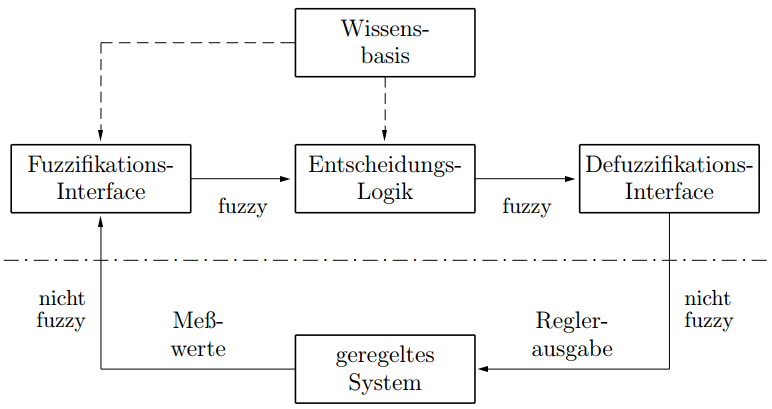
\includegraphics[width=0.7\linewidth]{../../../Downloads/fuzzyregler}
	\caption{Aufbau eines Fuzzy-Reglers.}
	\label{fig:fuzzyregler}
\end{figure}

\subsubsection{Wissensbasis}

Die Wissensbasis besteht aus der Regelbasis und Datenbasis. Alle Wertebreiche für die Eingangsgrößen sowie Stellgrößen $X_n, Y$ sowie die dazugehörigen linguistischen Termen sowie assoziierten Fuzzy-Mengen gehören zu der Datenbasis. Die Regelbasis besteht aus den linguistischen Kontrollregeln.

\subsubsection{Fuzzifizierungs-Interface}

Bei der sogennanten Fuzzifizierung geht es darum die kontinuirlichen analogen Eingangswerte aus den Definitionsmenge $X_n$ in eine Menge von Zugehorigkeitsgraden zu den Fuzzy-Mengen $F(X)$ umzuwandeln. Die Menge aller Zugehorigkeitsgrade zu $F(X)$ kann so als fuzziefizierte Eingangsgröße angesehen werden. Diese Einganggrößen verändern ihren Wert stetig wenn sich auch der analoge Eingangswert verändert. 

\subsubsection{Entscheidungslogik}

Die Entscheidungslogik versucht aus der bereits fuzzifizierten unscharfen Eingangsgröße eine unscharfe Ausgangsgröße oder Stellgröße abzuleiten. Dazu wird eine sogennante Regelbasis benötigt. Die Regelbasis besteht aus eine Menge von Kontrollregeln die meist von einem Domain-Experten aufgestellt werden.

\subsubsection{Defuzzyfizierungs-Interface}

Das Defuzzyfizierungs-Interface wandelt die Stellgröße, die in Form einer Fuzzy-Menge ausgedrückt wird, in einen scharfen Wert um. Dazu werden unterschiedliche Defuzzyfizierungs-Methoden verwendet. Die Methoden werden in Kapitel \ref{defuzzy} erläutert.


\subsection{Varianten der Fuzzy-Regelung}

Es haben sich zwei Arten von Fuzzy-Reglern etabliert. Zum einen gibt es den Ansatz von Mamdani und den Ansatz Takagi und Sugeno. Die auf Takagi und Sugeno zurückgehende Methode der Fuzzy-Regelung entspricht einer Modifizierung des Ansatzes von Mamdani.
Deshalb wird die Funktionsweise des Mamdani-Reglers zuerst erläutert.

Das allgemeine Entwurfsschema für einen Fuzzy Regler ist:

\begin{enumerate} 
	\item Festlegung der Ein- und Ausgangsgrößen.
	\item Festlegung der linguistischen Variablen durch Terme samt Zugehörigkeitsfunktionen
	für die in 1. eingeführten Größen.
	\item Erstellung der Regelbasis.
	\item Festlegung der Methoden zur Fuzzifizierung und Defuzzifizierung.
	\item Festlegung der Inferenzmethode.
\end{enumerate}

\subsubsection{Ansatz von Mamdani}

Bei diesem Ansatz formuliert der Experte des Systems eine Liste von $k$ verschiedenen linguistischen Regeln  der Form:

\begin{equation}
	\textbf{if} \; \xi_1 \; \textbf{is} \; A_{i1} \; \textbf{and... and} \; \xi_n \; \textbf{is} \; A_{in} \; \textbf{then} \; \eta \;\textbf{is} \;B
\end{equation}

Wobei $A_{i1},...,A_{in}$ und $B$ linguistische Terme sind. Diese müssen bereits vorher vom Experten des Systems bestimmt und den entsprechenden Fuzzy-Mengen zugeordnet werden. Diesen Vorgang nennt man auch Partitionierung. Dazu werden auf der Menge der Eingangsgrößen $X_n$ und der Ausgangsgröße $Y$ $p$ verschiedene Fuzzy-Mengen definiert und jede dieser Fuzzy-Mengen mit einem linguistischem Term zugeordnet. Hierzu können die in Kapitel \ref{representationsformen} vorgestellen Repräsentationsformen wie z.B. Dreiecksfunktionen oder Trapezfunktionen verwendet werden. Der Experte kann bei der Partitionierung entscheiden wie fein oder grob er den Wertebereich unterteilen möchte. Bei einer groben Partitionierung mit z.B. drei Fuzzy-Mengen benötigt man nicht viele Regeln und die Berechnung erfolgt schnell. Eine feinere Partitionierung mit fünf, sieben oder neun Fuzzy-Mengen liefert eine feinere Regelung. Häufig werden die Fuzzy-Mengen so gewählt, dass sie sich höchstens bis zu einem maximalen Grad von 0.5 überschneiden. Dies wird als Disjunktheitsforderung bezeichnet.

\newtheorem{disjunktheitsforderung}{Definition}
\begin{disjunktheitsforderung}
	Disjunktheitsforderung: $i \neq j \rightarrow sup_{x \in X} (min(\mu_i(x), \mu_k(x))}) \leq 0.5$
\end{disjunktheitsforderung}



% ----------------------------------------------------------------------------------------------------------



% Literatur



% ----------------------------------------------------------------------------------------------------------

\end{document}